\documentclass{article}
\usepackage[UTF8]{ctex}
\usepackage{graphicx}
\usepackage{fontspec}
\usepackage{xcolor}
\usepackage[vmargin=3cm]{geometry}
\begin{document}
\title{Lecture Notes 1}
\author{}
\date{\today}
\maketitle
\section{引言}
强化学习的目标是求解最优策略。
在此之前,我们需要一些工具来判断策略的好坏,以及什么是最优策略。
这些工具包括状态值、贝尔曼公式(Bellman equation)以及贝尔曼最优公式。 
接下来需要求解具体的策略和状态值,有很多不同的方法。
\section{第一章 基本概念}
\subsection{Grid World example: find a \textbf{good} way to the target}

\textbf{state}: 描述agent相对于environment的位置
\begin{figure}[htbp]
    \center{}
    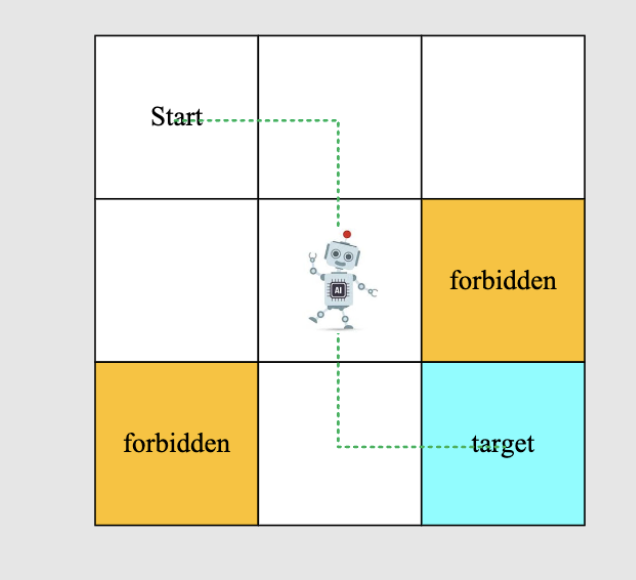
\includegraphics[width=0.5\textwidth]{picture1.png}
    \center{}
\end{figure}

\textbf{state space}:状态的集合

\textbf{action}: 不同的状态可能有不同的action。

\textbf{action space}: action的集合。行动空间是状态空间的一个函数,因为不同的状态可能具有不同的行动。

\textbf{state transition}:状态转移,在某状态时采取某行动会导致状态的转移。具体转移到哪个状态取决于状态空间

\textcolor{blue}{\kaishu*用概率描述状态转移是一种普适的方法}

\textbf{policy}: 描述agent到了某个状态会实行某个策略,同样是以条件概率的形式

\begin{figure}[htbp]
    \center{}
    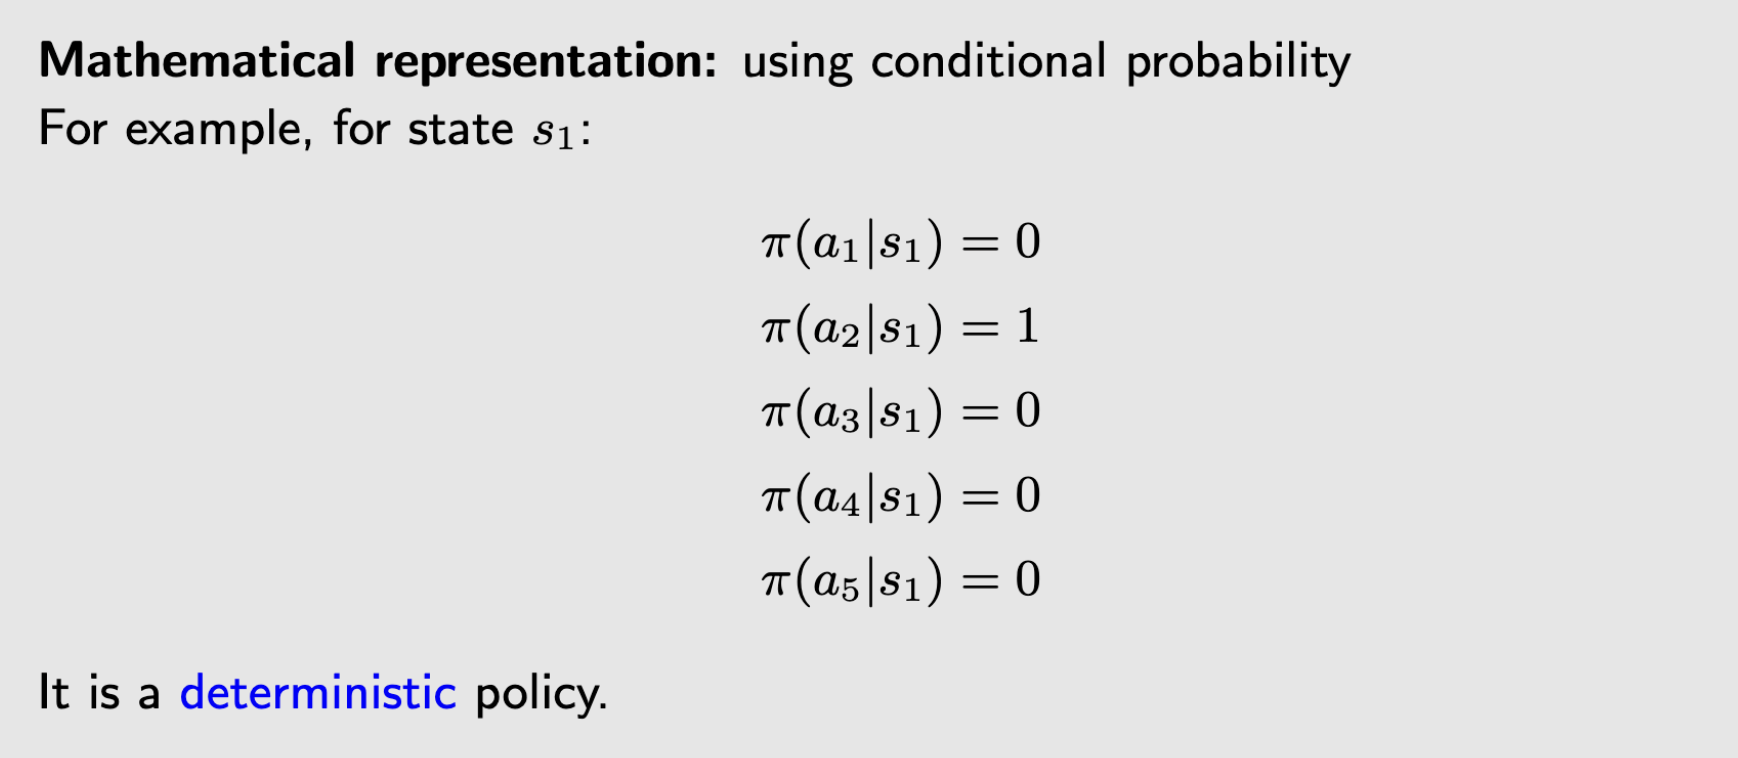
\includegraphics[width=0.6\textwidth]{picture3.png}
    \center{}
\end{figure}

\textbf{reward}:根据agent的行动结果作出奖励或者惩罚。agent会尽量最大化奖励和最小化惩罚。同样可以使用条件概率进行表示

\textcolor{blue}{\kaishu*reward可以视为人类与agent交互的一种手段}

\textbf{trajectory}: a state-action-reward transition

\textbf{return}: 计算沿着某个trajectory到达target时agent获得了多少奖励,可以用来评估trajectory的好坏

\textbf{discount rate}:衰减率,$\gamma \in [0, 1)$。通过调整$\gamma$,可以促使agent采取不同的策略。$\gamma$ 越小,agent就越近视。反之,则越远视。

\textbf{episode}:一整个从开始到target的过程称为一个episode。有限步数的任务称为episodic task,而无限步数的任务称为continuing task。

\textcolor{blue}{\kaishu*将episodic task 转化为continuing task的方法:将target节点一般化,不视为最终节点,到达后可以进行移动}

\end{document}